
%!TEX ROOT=DavidPetrDP.tex
\chapter{Úvod}
V rámci výuky na katedře měření v předmětech zaměřující se na elektroniku se již nějaký čas používají softwarově definované přístroje(SDI), které slouží jako dostupná náhrada za laboratorní vybavení jako jsou osciloskopy nebo signálové generátory. Ač tyto přístroje nedosahují parametrů profesionálních přístrojů, tak existuje mnoho aplikací, kde jejich výkon ve smyslu maximální vzorkovací frekvence či přesnosti určení napětí je dostatečné a přístroje tak mohou v těchto případech profesinální přístroje nahradit.\\

Konkrétně v předmětu laboratoře průmyslové elektroniky(LPE) se právě používá SDI běžící na MCU STM32F042 v kombinaci s aplikací Zero Elab Viewer pro různé experimenty jako je měření časové konstanty RC článku, zapojování různých obvodů s operačními zesilovači a mnoho dalších. SDI se v rámci výuky také používá pro diagnostiku správnosti funkce programů, které studenti sami programují na výukových modulech s nepájivými poli.\\

Nově se studenti učí programovat MCU řady STM32G431, které oproti původně používanému MCU STM32F042 nabízí vyšší výpočetní výkon a také nové periferie jako je například DAC převodník. Vhodnost využití tohoto MCU jakožto SDI již ukázala dříve vzniklá implementace SDI na tomto MCU spolupracující s aplikací VSVI, která také vznikla zde na fakultě. Ovládání této aplikace se ale prokázalo méně intuitivní než je tomu v případě Zero Elab Viewer a zároveň studenti stále v těchto využívají hotový modul s STM32F042 a tak vznikla myšlenka využít STM32G431 k implementace SDI spolupracují Zero Elab Viewer a přidat rozšířit funkcionalitu pro studenty a vyučující známé aplikaci.


\chapter{Rozbor}
Jak již bylo výše zmíněno v laboratoři se dlouhodobě používá SDI vzniklý okolo STM32F042 společně s aplikací Zero Elab Viewer. V rámci výuky programování mikrokontrolérů se přešlo na nový modul(obr. \ref{fig:g431breadboard}) s výkonnějším MCU STM32G431, který obsahuje jádro ARM Cortex-M4 a vyšší počet periferií než doposud používaná STM32F042. Otevřely se tím možnosti pro implementace SDI s lepšími parametry, jako je například modul vzniklý v rámci práce \cite{DujavaDIP} spolupracující s aplikací VSVI. Ten oproti dosud používanému řešení nabízel nově funkční generátor, komplexní pulzní generátor a také výrazně vyšší vzorkovací frekvence osciloskopu dosahující až 6.5 MSps.

\begin{figure}[H]
	\centering
	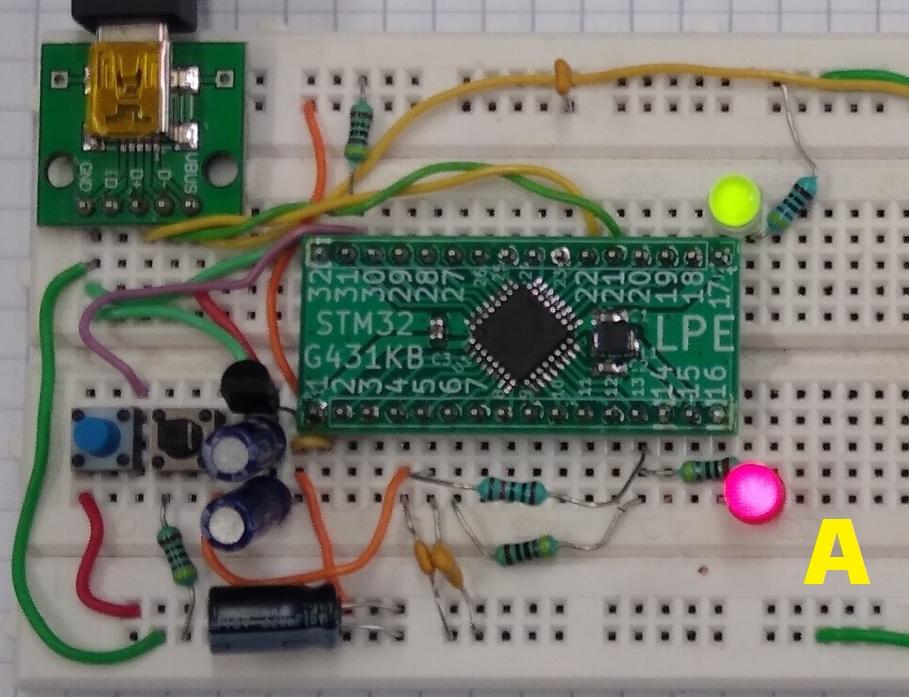
\includegraphics[width=0.5\linewidth]{Figs/Documentation/G431breadboard}
	\caption{Modul s STM32G431 na nepájivém poli používaný v rámci výuky LPE, převzato z \cite{LPE}}
	\label{fig:g431breadboard}
\end{figure}

Nicméně jiné ovládání (TUI) oproti klasickému grafickému rozhraní a také vyšší komplexnost tohoto řešení způsobili horší uživatelskou zkušenost a vznikla poptávka po vytvoření FW pro STM32G431, který by spolupracoval s původní aplikací Zero Elab Viewer a zároveň přinášel zlepšení parametrů jako maximální vzorkovací frekvence a rozšíření funkcionalit. Zároveň studenti mají k dispozici modul (obr. \ref{fig:modulef042}) pro méně náročná měření, a tedy v případě přecházení od jedné implementace SDI k druhé by pak odpadala nutnost se orientovat v novém prostředí. 
\begin{figure}[H]
	\centering
	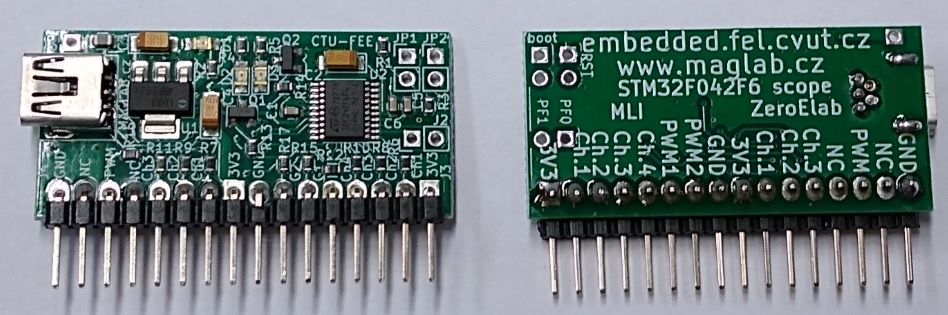
\includegraphics[width=0.7\linewidth]{Figs/Documentation/module_F042}
	\caption{Modul SDI s STM32F042 s předchystaným FW pro Zero Elab Viewer    }
	\label{fig:modulef042}
\end{figure}
Úkolem této práce tedy je vytvořit firmware pro mikrořadič STM32G431 tak, aby jej ve spolupráci
s PC aplikací Zero eLab Viewer bylo možno využít jako jednoduchý, avšak komplexní měřicí přístroj pro výukové účely. Nejdříve bylo nutno tedy analyzovat protokol existující aplikace a vytvořit firmware tak, aby využil všech funkcí, které aplikace již nabízí. Dále by mělo dojít ke zlepšení parametrů oproti původní verzi SDI pro STM32F042 a to především dosáhnout vyšších vzorkovacích frekvencí osciloskopu a logického analyzátoru, využít větších paměťových kapacit, které STM32G431 nabízí pro  delší záznamovou paměť a v neposlední řadě také implementovat nové funkce jako je generátor funkcí. Přístroj by měl dále zahrnovat funkce impulsního generátoru, čítače a voltmetru se záznamem.
\section{PC aplikace Zero Elab Viewer}
V roce 2016 v rámci své diplomové práce \cite{BerlingerDIP} pan Ing.Adam Berlinger vytvořil aplikaci Zero Elab Viewer fungující jako grafické rozhraní pro komunikaci se softwarově definovaným nástrojem(SDI) založeném na STM32F042. Aplikace společně s FW umožňuje používání MCU jako dostupnou náhradu za laboratorní přístroje  jako jsou voltmetr, osciloskop, impulsní generátor, signálový generátor nebo logický analyzátor. Aplikace se od té doby stále používá ve výuce praktické elektroniky a od té doby vznikla ještě řada implementací FW pro jiné MCU. Nejnověji například verze pro mikrokontrolér ATMega 328 pro uživatele se zkušenostmi s ARDUINO nebo zatím nejmenší (a nejlevnější) varianta SDI přístoje vzniklá využívající 8-pinovou variantu mikrokontroleru STM32G030.\\

\begin{figure}[H]
	\centering
	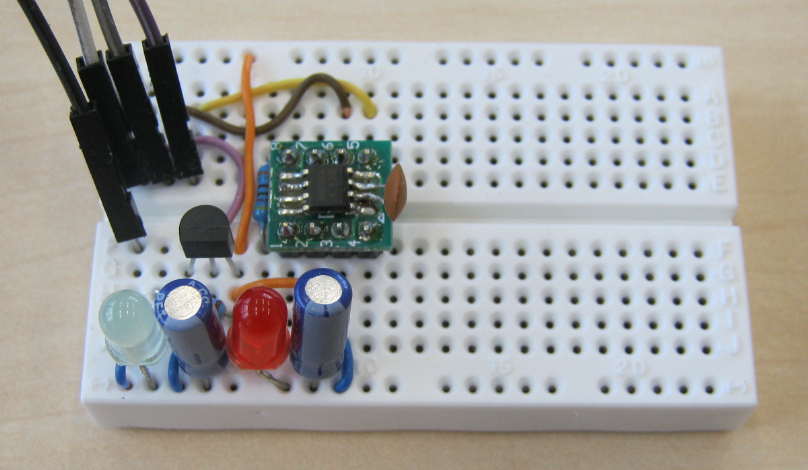
\includegraphics[width=0.5\linewidth]{Figs/Screenshots/G0_Lab_foto2}
	\caption{STM32G031 zapojen na nepájivém poli převzato z \cite{G030Foto}}
	\label{fig:g0labfoto2}
\end{figure}

\subsection{Existující SDI FW pro spolupráci s aplikací Zero Elab Viewer}

\begin{itemize}
	\item Firmware pro SDI s STM32F042
	\begin{itemize}
		\item Osciloskop- záznam až 1152 vzorků, rozlišení 12 bitů,
		\item Rychlost záznamu až 1x 600 kS/s 
		\item Ve stroboskopickém módu - až  48 MS/s - rozlišení s intervalem 15,6 ns.
		\item Impulsní generátor PWM , nastavení  střídy 0 až 100 \%; nastavení frekvence 1 Hz až 24 MHz
		\item Voltmetr tři kanály, 0 až + 3,3 V, 100 odměrů/s, průměrování z 1 až 256 odměrů, možnost funkce záznamu
	\end{itemize}
	\item Firmware pro SDI STM32G030
	\begin{itemize}
		\item Osciloskop- záznam až 2048 vzorků, rozlišení 12 bitů,
		\item Rychlost záznamu až 1x 2 MS/s (nebo  2x 1 MS/s, 3 x 666 kS/s).
		\item Ve stroboskopickém módu - až  64 MS/s - rozlišení s intervalem 15,6 ns.
		\item Impulsní generátor PWM , nastavení  střídy 0 až 100 \%; nastavení frekvence 1 Hz až 32 MHz
		\item Voltmetr tři kanály, 0 až + 3,3 V, 100 odměrů/s, průměrování z 1 až 256 odměrů, možnost funkce záznamu
	\end{itemize}
	\item Firmware pro SDI s ATMega 328
			\begin{itemize}
		\item Dvoukanálový Osciloskop- záznam až 768 vzorků, rozlišení 8 bitů,
		\item Rychlost záznamu až 1x 80 kS/s (nebo  2x 50 kS/s, 3 x 666 kS/s).
		\item Ve stroboskopickém módu - až  4 MS/s - rozlišení s intervalem 250 ns.
		\item Impulsní generátor PWM , nastavení  střídy 0 až 100 \%; nastavení frekvence 0.5 Hz až 4 MHz
		\item Voltmetr tři kanály, 0 až +5 V, rozlišení 10 bitů, 100 odměrů/s, průměrování z 1 až 256 odměrů, možnost funkce záznamu
	\end{itemize}
	
\end{itemize}

\section{Použitý MCU STM32G431}
Navržený mikrokontrolér s jádrem Arm® 32-bit Cortex®-M4 může běžet až s maximální frekvencí jádra 170MHz a tak ve srovnání s předchozími implementacemi na STM32F042(48MHz) a STM32G030(64MHz) nabízí větší výpočetní výkon. Navíc obsahuje více dostupných periferií vhodným pro implementaci SDI, jako jsou 2 ADC převodníky či větší počet periferií čítačů(14 vs 8 u G030).

\section{Komunikační protokol aplikace ZeroElab Viewer }
Komunikační protokol aplikace Zero Elab Viewer je postaven kolem 2 druhů zpráv. Druhy zpráv jsou od sebe navzájem odlišeny prvním bytem zprávy. Zaprvé jsou to zprávy typu příkazů, (CMD), které slouží k oboustrannému předávání pokynů. Jedná se o jednoduché zprávy, ve kterých pole CH určuje, kterému modulu je příkaz určen, tedy jestli se jedná o příkaz voltmetru, pulzního generátoru nebo například obecný příkaz měnící konfiguraci přístroje. Dále pole CMD rozlišuje, o jaký druh příkazu se jedná. Typicky příkaz společný pro jednotlivé moduly je zapnutí/vypnutí běhu daného modulu a hodnota příkazu pak rozšiřuje možnost předaných parametrů spojených s daným příkazem. Druhým typem zpráv jsou je data, která míří z MCU do aplikace v PC specifikovaná číslem kanálu(modulu), z kterého data pocházejí, délkou data po které pak už následují samotná data. Oba formáty zpráv jsou naznačeny na obrázcích \ref{fig:communicationcmd} a \ref{fig:communicationdata}. 
 
\begin{figure}[H]
	\centering
	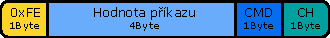
\includegraphics[width=0.7\linewidth]{Figs/Diagrams/SVG/CommunicationCMD.pdf}
	\caption{Rozložení bytů ve zprávě typu příkaz(CMD)}
	\label{fig:communicationcmd}
\end{figure}

\begin{figure}[H]
	\centering
	
\includegraphics[width=0.7\linewidth]{Figs/Diagrams/SVG/CommunicationDATA.pdf}
	\caption{Rozložení bytů ve zprávě typu data}
	\label{fig:communicationdata}
\end{figure}

